\documentclass[11pt]{article}
\usepackage[margin=1in]{geometry}
\usepackage[T1]{fontenc}
\usepackage[utf8]{inputenc}
\usepackage{lmodern}
\usepackage{microtype}
\usepackage{amsmath,amssymb}
\usepackage{booktabs}
\usepackage{graphicx}
\usepackage{xcolor}
\usepackage{tikz}
\usepackage[numbers]{natbib}
\usepackage{hyperref}
\usepackage{float}
\usetikzlibrary{arrows.meta,positioning,calc}

\hypersetup{colorlinks=true, linkcolor=blue, citecolor=blue, urlcolor=blue}

\title{Intervention-Aware World Models for Agents: Real-Data Tests of the Causal World Encoder}
\author{Kunj Rathod\\University of Utah}
\date{}

\begin{document}
\maketitle

\begin{abstract}
This paper asks a narrower question than most world-model papers: if an agent needs to reason about interventions rather than just observations, which architectural bias actually helps at small scale on real data? We study a proposed Causal World Encoder (CWE) with three components: a hierarchical timescale belief state (HTBS), a twin-stream intervention-conditioned predictor (TICP), and a sparse predictive commitment gate (SPCG). Unlike many architectural proposals, the paper uses only public real datasets and reproducible laptop-scale experiments. On 1,986 LoCoMo questions over 5,882 dialogue memories, lexical retrieval remains strongest at Hits@5 (0.3197) and the hybrid ranker only narrowly improves Hits@10 (0.3933 vs. 0.3922), underscoring how much long-horizon memory still depends on exact evidence spans. On an eight-document workflow built from live arXiv abstracts, bounded workspace reconstruction reduces cumulative prompt load by 69.23\% while preserving complete title and keyword coverage. On BabyAI offline trajectories, TICP improves held-out-action cosine from 0.4046 to 0.4224 and local Top-1 from 0.3003 to 0.3271; a follow-up across three held-out action splits shows the same pattern each time, with held-out cosine gains of 0.0178, 0.0131, and 0.0211. The more ambitious CWE claims receive mixed support: HTBS is competitive but not dominant, and SPCG successfully budgets computation while only partially separating high-change from routine transitions. The honest conclusion is therefore selective rather than grandiose: explicit action/world decomposition is the strongest part of the proposal, bounded external state remains useful, and the current HTBS/SPCG designs need more work before they justify stronger architectural claims.
\end{abstract}

\section{Introduction}
The core weakness of standard sequence modeling for agents is not merely that context windows are finite. It is that most models are trained to be good at observation-conditioned prediction while agents ultimately need intervention-sensitive prediction. A next-token transformer, and even a latent predictor in the JEPA family, can be very good at estimating what tends to happen after a state. That is not the same thing as isolating what happened because the agent acted. For planning, repair, and counterfactual evaluation, that distinction matters.

A second weakness is temporal organization. Long-horizon agent systems either replay large amounts of history through attention or compress everything into an opaque recurrent state. The former scales badly with horizon; the latter can hide exactly the distinctions the agent later needs. This motivates a structured alternative: multiscale compression for state, an explicit decomposition between passive dynamics and action-conditioned change, and a budgeted mechanism for deciding when a predictive update is worth committing.

This paper evaluates that design hypothesis rather than selling a frontier-scale system. The proposed Causal World Encoder (CWE) combines three ideas. HTBS organizes memory into slots that update on different clocks. TICP decomposes next-state prediction into a state-only dynamics term and an action-conditioned residual. SPCG allows the model to defer predictive updates unless a state appears worth committing. The center of gravity is TICP, because it is the only component that directly attacks the observation-versus-intervention mismatch and, in the experiments below, it is the one that consistently survives contact with real data.

The empirical stance is intentionally conservative. We do not claim a general replacement for transformers, a complete structural causal model, or large-scale embodied competence. We ask a simpler question: which architectural effects remain visible on real public datasets when the entire project must fit on a laptop and all results must be reproducible? The answer is mixed in exactly the way a useful systems paper should be mixed: bounded state helps, lexical retrieval remains surprisingly important, twin-stream action decomposition helps, and the more ambitious multiscale and sparse-gating components are promising but not yet dominant.

\paragraph{Contributions.}
\begin{enumerate}
    \item We formalize CWE as a modular intervention-aware extension of bounded-state agent architecture, separating multiscale belief compression, action-effect decomposition, and sparse predictive commitment.
    \item We run six real-data experiments: LoCoMo retrieval, a live arXiv bounded-workspace benchmark, a main held-out-action BabyAI experiment, a sequence-model comparison across temporal horizons, a sparse commitment analysis, and a focused TICP follow-up across three alternative held-out action splits.
    \item We report a deliberately honest result profile: action/world decomposition is the clearest win, bounded workspace remains useful, lexical retrieval is stronger than fashionable dense baselines on LoCoMo, and the present HTBS/SPCG instantiations do not earn a superiority claim.
\end{enumerate}

\section{Problem Setting and Design Requirements}
Let $s_t$ denote an agent's latent or structured state, $a_t$ an action, $M_t$ persistent memory, and $C_t$ a bounded prompt context reconstructed from state and memory. We care about four requirements.
\begin{description}
    \item[R1: Persistence.] Relevant information should survive beyond the active prompt.
    \item[R2: Boundedness.] Context should scale with task state, not transcript length.
    \item[R3: Intervention sensitivity.] The architecture should distinguish state changes attributable to the world from state changes attributable to actions.
    \item[R4: Practicality.] Informative experiments should run on commodity hardware before any large-scale training claim is made.
\end{description}

The first two requirements motivate the retrieval and workspace experiments. The third motivates the twin-stream decomposition. The fourth constrains every implementation choice in the repo.

\section{Related Work}
JEPA-style learning replaces observation reconstruction with prediction in representation space, which can produce more abstract targets than next-token modeling \citep{assran2023jepa, chen2025vljepa, assran2025vjepa2}. Persistent memory systems such as Hindsight and long-horizon frameworks such as InfiAgent argue that agents need structured state external to the transcript \citep{latimer2025hindsight, yu2026infiagent}. LoCoMo sharpened the retrieval side of that claim by constructing a benchmark around very long conversational memory \citep{maharana2024locomo}. Verified tool-use systems such as ToolGate provide a complementary lesson: if state changes matter, committing them blindly is a bad idea \citep{liu2026toolgate}.

\subsection{State-space models and recurrent alternatives}
Recent sequence-model work has re-opened the question of whether full self-attention is the right primitive for long-horizon state tracking. Mamba uses selective state spaces to achieve linear-time sequence modeling while preserving strong empirical performance \citep{gu2023mamba}. Griffin mixes gated linear recurrences with local attention, again suggesting that long-range compression and local access need not be handled by the same mechanism \citep{de2024griffin}. Older multiscale recurrent ideas such as Clockwork RNNs make the same point in a cleaner form: different timescales may deserve different update schedules \citep{koutnik2014clockwork}. CWE's HTBS borrows this intuition, though the experiments here show that the benefit is far from automatic.

\section{Architecture}
Figure~\ref{fig:modular-architecture} gives the broader bounded-state agent picture, while Figure~\ref{fig:cwe-architecture} shows the specific CWE extension.

\begin{figure}[t]
\centering
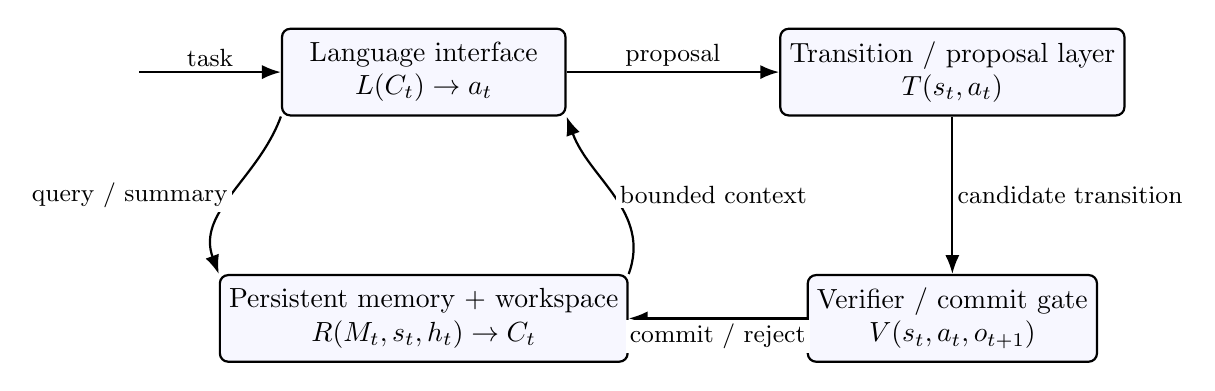
\begin{tikzpicture}[
    node distance=2.0cm and 2.7cm,
    module/.style={draw, rounded corners=3pt, thick, minimum width=3.6cm, minimum height=1.1cm, align=center, fill=blue!3},
    flow/.style={-{Latex[length=2.4mm]}, thick},
    lab/.style={font=\small, fill=white, inner sep=1.5pt, align=center}
]
\node[module] (lang) {Language interface\\$L(C_t) \to a_t$};
\node[module, right=of lang] (pred) {Transition / proposal layer\\$T(s_t, a_t)$};
\node[module, below=of lang] (mem) {Persistent memory + workspace\\$R(M_t, s_t, h_t) \to C_t$};
\node[module, below=of pred] (ver) {Verifier / commit gate\\$V(s_t, a_t, o_{t+1})$};
\draw[flow] ([xshift=-1.8cm]lang.west) -- node[lab, above] {task} (lang.west);
\draw[flow] (lang.east) -- node[lab, above] {proposal} (pred.west);
\draw[flow] (pred.south) -- node[lab, right] {candidate transition} (ver.north);
\draw[flow] (ver.west) -- node[lab, below] {commit / reject} (mem.east);
\draw[flow] (mem.north east) to[out=70,in=-70] node[lab, right] {bounded context} (lang.south east);
\draw[flow] (lang.south west) to[out=-110,in=110] node[lab, left] {query / summary} (mem.north west);
\end{tikzpicture}
\caption{Bounded-state agent architecture. Language proposes; memory reconstructs context; a transition layer predicts or ranks futures; and a verifier decides what becomes trusted state.}
\label{fig:modular-architecture}
\end{figure}

\subsection{Hierarchical Timescale Belief State}
HTBS keeps $K$ slots with update periods $2^0,2^1,\ldots,2^{K-1}$. Slot $k$ updates only when the clock for that slot fires:
\[
 s_k(t) = \begin{cases}
 \mathrm{GRU}_k\left(s_k(t-2^k), \operatorname{pool}(x_{t-2^k:t})\right), & t \equiv 0 \pmod{2^k} \\
 s_k(t-1), & \text{otherwise.}
 \end{cases}
\]
The final belief state is the concatenation of slot states. This gives structured temporal compression, but the results below show that structured compression alone does not guarantee better next-state decoding.

\subsection{Twin-Stream Intervention-Conditioned Predictor}
TICP factorizes prediction into a state-only term and an action-conditioned residual:
\[
 z^{world}_{t+1} = f_{dyn}(s_t), \qquad z^{delta}_{t+1} = f_{int}(s_t, a_t), \qquad \hat z_{t+1} = z^{world}_{t+1} + z^{delta}_{t+1}.
\]
This does not make the model a full structural causal model in Pearl's sense. It does make intervention effects an explicit architectural object, which is enough to test whether action/world factorization helps generalization.

\subsection{Sparse Predictive Commitment Gate}
SPCG predicts both a next-state proposal and a gate probability $g_t \in [0,1]$. The committed prediction is a mixture of the predictor output and a carry-forward state:
\[
 \hat s_{t+1} = g_t \, f(s_t, a_t) + (1-g_t) s_t.
\]
A budget penalty keeps the mean gate probability near a target rate. The attractive cognitive-science story comes from active inference and event segmentation \citep{friston2017active, zacks2007perception, zacks2007segmentation}, but the experiment below shows only weak evidence for clean event-boundary specialization.

\begin{figure}[t]
\centering
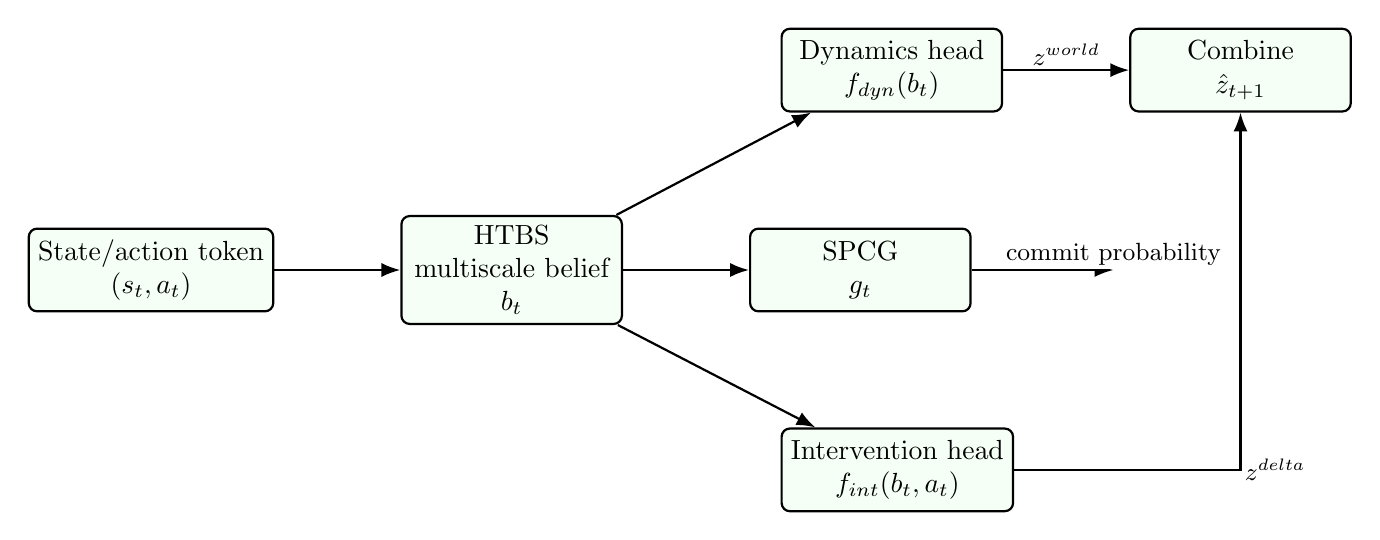
\begin{tikzpicture}[
    node distance=1.9cm and 1.6cm,
    module/.style={draw, rounded corners=3pt, thick, minimum width=2.8cm, minimum height=1.05cm, align=center, fill=green!4},
    flow/.style={-{Latex[length=2.4mm]}, thick},
    lab/.style={font=\small, fill=white, inner sep=1.2pt, align=center}
]
\node[module] (state) {State/action token\\$(s_t, a_t)$};
\node[module, right=of state] (htbs) {HTBS\\multiscale belief\\$b_t$};
\node[module, above right=1.3cm and 2.0cm of htbs] (dyn) {Dynamics head\\$f_{dyn}(b_t)$};
\node[module, below right=1.3cm and 2.0cm of htbs] (int) {Intervention head\\$f_{int}(b_t,a_t)$};
\node[module, right=of htbs] (gate) {SPCG\\$g_t$};
\node[module, right=of dyn] (sum) {Combine\\$\hat z_{t+1}$};
\draw[flow] (state) -- (htbs);
\draw[flow] (htbs) -- (dyn);
\draw[flow] (htbs) -- (int);
\draw[flow] (htbs) -- (gate);
\draw[flow] (dyn) -- node[lab, above] {$z^{world}$} (sum);
\draw[flow] (int.east) -| node[lab, right] {$z^{delta}$} (sum.south);
\draw[flow] (gate.east) -- ++(1.8,0) node[lab, above] {commit probability};
\end{tikzpicture}
\caption{CWE components. HTBS compresses multiscale context, TICP separates state-only dynamics from action-conditioned deltas, and SPCG decides how strongly to commit a predictive update.}
\label{fig:cwe-architecture}
\end{figure}

\section{Experiments}
All experiments use real public data. Retrieval uses the released LoCoMo text benchmark. The bounded-workspace test fetches eight live arXiv abstracts. The intervention, timescale, and sparse-commitment experiments use offline BabyAI trajectories from public Minari mirrors on Hugging Face. Training ran on CPU for numerical stability and reproducibility.

\subsection{Experiment 1: Conversational retrieval on LoCoMo}
We flatten the LoCoMo release into 5,882 dialogue-turn memories and 1,986 question/evidence pairs. We compare TF--IDF, dense MiniLM retrieval, and reciprocal-rank-fusion hybrid retrieval. Metrics are Hits@1, Hits@5, Hits@10, MRR, and nDCG@10.

\subsection{Experiment 2: Bounded-workspace reconstruction on live abstracts}
We fetch eight real arXiv abstracts spanning agent memory, sequence modeling, and world models. At each step the system records a structured note with title, claim sentence, and extracted keywords. We compare a full-transcript prompt to a bounded workspace reconstructed from notes plus the two most recent actions. The metric is prompt size and cumulative prompt load, with exact title and keyword coverage as a fidelity check.

\subsection{Experiment 3: Intervention decomposition on BabyAI trajectories}
We use offline trajectories from BabyAI-KeyCorridorS3R1 and BabyAI-UnlockPickup. Actions $\{0,1,2,4\}$ (left, right, forward, drop) are used for training; pickup and toggle ($\{3,5\}$) are held out. Action representations are MiniLM sentence embeddings of action names so that zero-shot transfer has at least a semantic route. We compare a single-stream MLP against TICP on cosine similarity and local nearest-neighbor decoding.

\subsection{Experiment 4: Timescale factorization versus flat alternatives}
From the same BabyAI trajectories we build sequence examples of lengths 4, 8, 12, and 16. Each timestep concatenates the current state feature vector with an action embedding; the target is the next state feature vector. We compare HTBS, an LSTM, a 2-layer causal transformer, and a per-step MLP control.

\subsection{Experiment 5: Sparse commitment versus dense prediction}
A dense predictor always updates the next state. SPCG learns a gate probability and is evaluated with a threshold chosen to realize the target commitment rate of 30\%. We report overall prediction quality, committed-subset quality, and whether the gate prefers genuinely higher-change steps.

\subsection{Experiment 6: Focused TICP follow-up across held-out action splits}
To stress-test the strongest component of CWE, we rerun the intervention experiment across three held-out action splits rather than only one: pickup+toggle, turning, and forward+drop. In each condition, the model trains on the remaining four actions and is evaluated only on held-out actions from the test episodes. The point is not to manufacture a heroic benchmark; it is to test whether the twin-stream advantage survives when the held-out actions change.

\section{Results}
\subsection{LoCoMo retrieval}
\begin{table}[H]
\centering
\caption{LoCoMo retrieval on 1,986 questions and 5,882 memories.}
\begin{tabular}{lccccc}
\toprule
Method & Hits@1 & Hits@5 & Hits@10 & MRR & nDCG@10 \\
\midrule
TF--IDF & 0.1677 & 0.3197 & 0.3922 & 0.2341 & 0.2562 \\
Dense MiniLM & 0.0851 & 0.2190 & 0.2925 & 0.1435 & 0.1679 \\
Hybrid RRF & 0.1219 & 0.2976 & 0.3933 & 0.1991 & 0.2307 \\
\bottomrule
\end{tabular}
\label{tab:retrieval}
\end{table}

\begin{figure}[H]
\centering
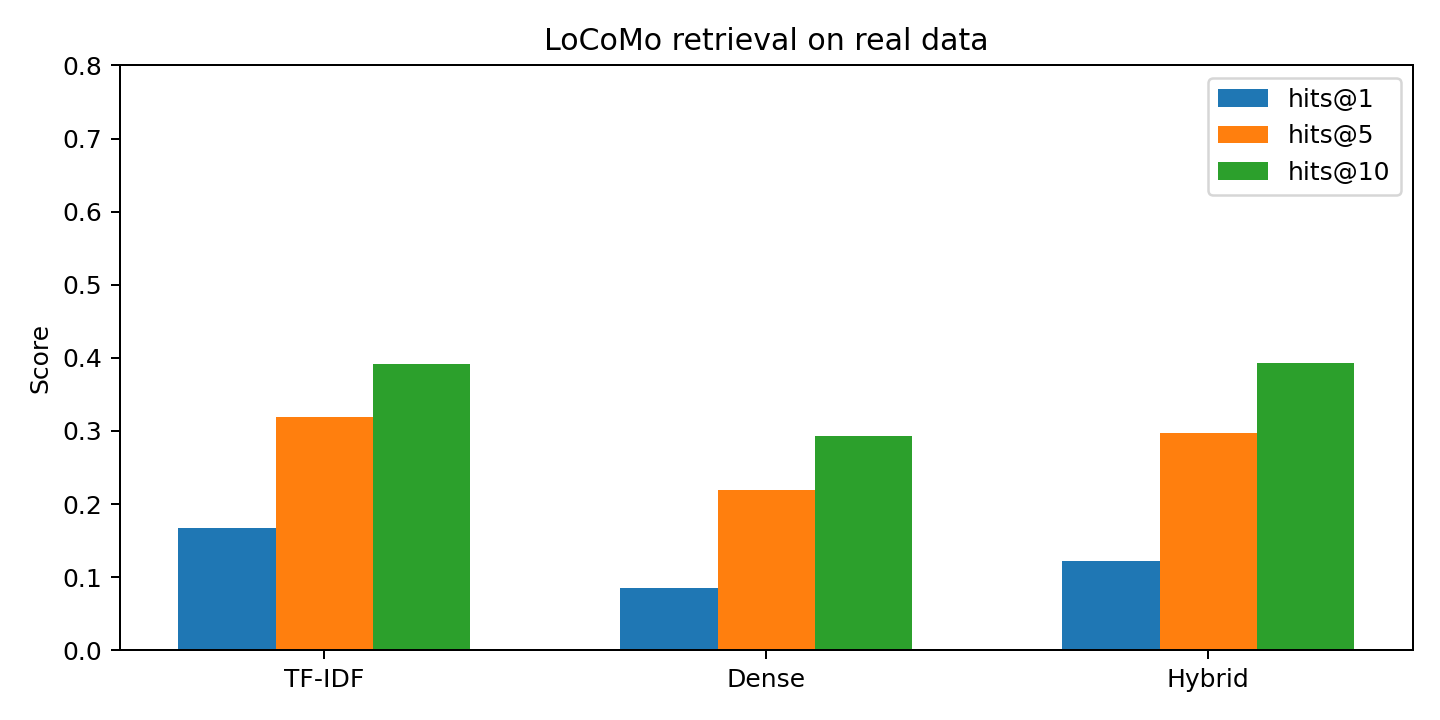
\includegraphics[width=0.82\linewidth]{../results/figures/exp1_retrieval.png}
\caption{LoCoMo retrieval with real released data. Lexical retrieval remains strongest at shallow recall and the hybrid only barely edges TF--IDF at Hits@10.}
\label{fig:retrieval}
\end{figure}

The retrieval result is more interesting because it is not flattering to the fashionable baseline. Dense MiniLM retrieval is consistently weaker than TF--IDF. Hybrid fusion recovers some of that loss and slightly improves Hits@10, but not enough to beat lexical retrieval at Hits@5. The practical lesson is that long-horizon conversational memory is still heavy on exact names, dates, and surface anchors.

\subsection{Bounded workspace}
\begin{table}[H]
\centering
\caption{Prompt growth on a live eight-document arXiv workflow.}
\begin{tabular}{lcc}
\toprule
Metric & Full transcript & Bounded workspace \\
\midrule
Final prompt size (chars) & 12321 & 2830 \\
Cumulative prompt load (chars) & 54521 & 16775 \\
Title coverage & 1 & 1 \\
Keyword coverage & 1 & 1 \\
\bottomrule
\end{tabular}
\label{tab:workspace}
\end{table}

\begin{figure}[H]
\centering
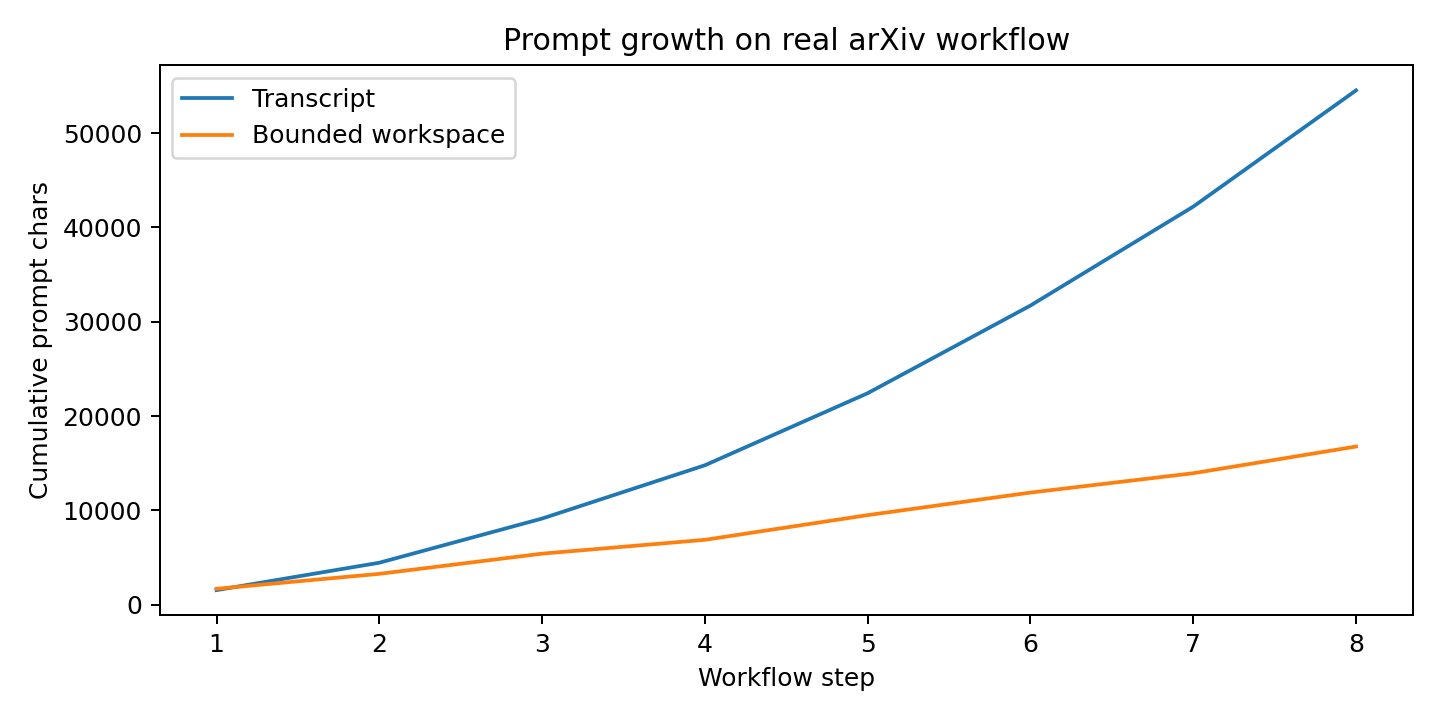
\includegraphics[width=0.82\linewidth]{../results/figures/exp2_workspace.png}
\caption{Cumulative prompt growth for the live arXiv workflow.}
\label{fig:workspace}
\end{figure}

Bounded workspace reconstruction cuts final prompt size by 77.03\% and cumulative prompt load by 69.23\% while preserving exact title and keyword coverage. This is not a full interactive agent benchmark, but it is a clean real-data confirmation that externalized workspace state changes scaling behavior materially.

\subsection{Intervention decomposition}
\begin{table}[H]
\centering
\caption{Held-out-action generalization on BabyAI offline trajectories.}
\begin{tabular}{lcccc}
\toprule
Model & Seen cosine & Held-out cosine & Held-out Top-1 & Held-out Top-5 \\
\midrule
Single-stream & 0.5399 & 0.4046 & 0.3003 & 1.0000 \\
Twin-stream & 0.5530 & 0.4224 & 0.3271 & 1.0000 \\
\bottomrule
\end{tabular}
\label{tab:intervention}
\end{table}

\begin{figure}[H]
\centering
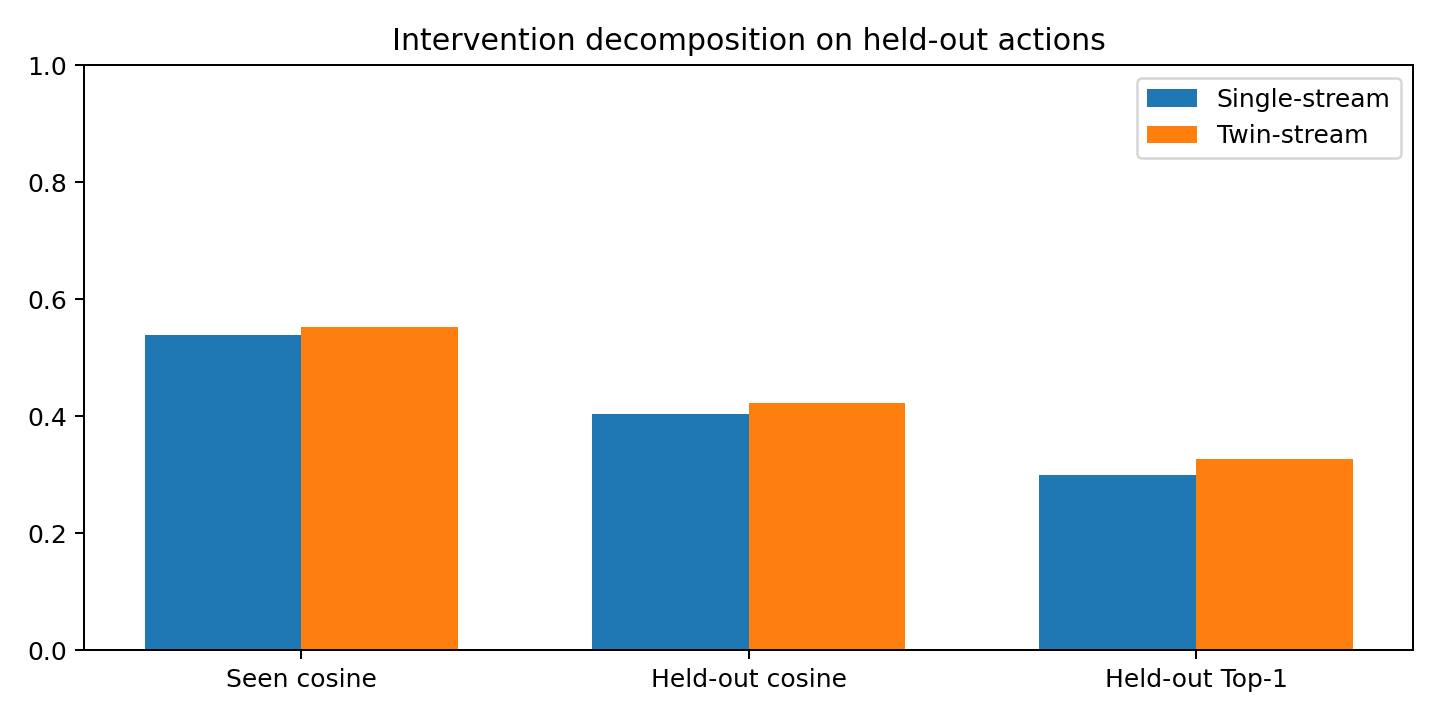
\includegraphics[width=0.82\linewidth]{../results/figures/exp3_intervention.png}
\caption{Twin-stream decomposition improves held-out-action cosine and local Top-1, although the gain is modest.}
\label{fig:intervention}
\end{figure}

This is the cleanest positive result for CWE. On held-out actions, the twin-stream model improves cosine by 0.0178 and local Top-1 by 0.0268. The effect is not huge, but it is consistent with the core thesis that separating state-only dynamics from action-conditioned deltas is a better inductive bias than a single undifferentiated predictor.

\subsection{Timescale factorization}
\begin{table}[H]
\centering
\caption{Sequence-model comparison across episode lengths.}
\begin{tabular}{lcccc}
\toprule
Length & Best model (Top-1) & Best Top-1 & Best Top-5 & Best train seconds \\
\midrule
4 & MLP control & 0.3327 & 0.6041 & 2.15 \\
8 & Transformer & 0.3478 & 0.6500 & 27.39 \\
12 & MLP control & 0.3542 & 0.7205 & 1.11 \\
16 & Transformer & 0.4369 & 0.8702 & 12.08 \\
\bottomrule
\end{tabular}
\label{tab:timescale-summary}
\end{table}

\begin{table}[H]
\centering
\caption{HTBS versus transformer on local Top-1.}
\begin{tabular}{lcc}
\toprule
Length & HTBS Top-1 & Transformer Top-1 \\
\midrule
4 & 0.2742 & 0.3151 \\
8 & 0.3115 & 0.3478 \\
12 & 0.2844 & 0.3392 \\
16 & 0.3303 & 0.4369 \\
\bottomrule
\end{tabular}
\label{tab:timescale-htbs}
\end{table}

\begin{figure}[H]
\centering
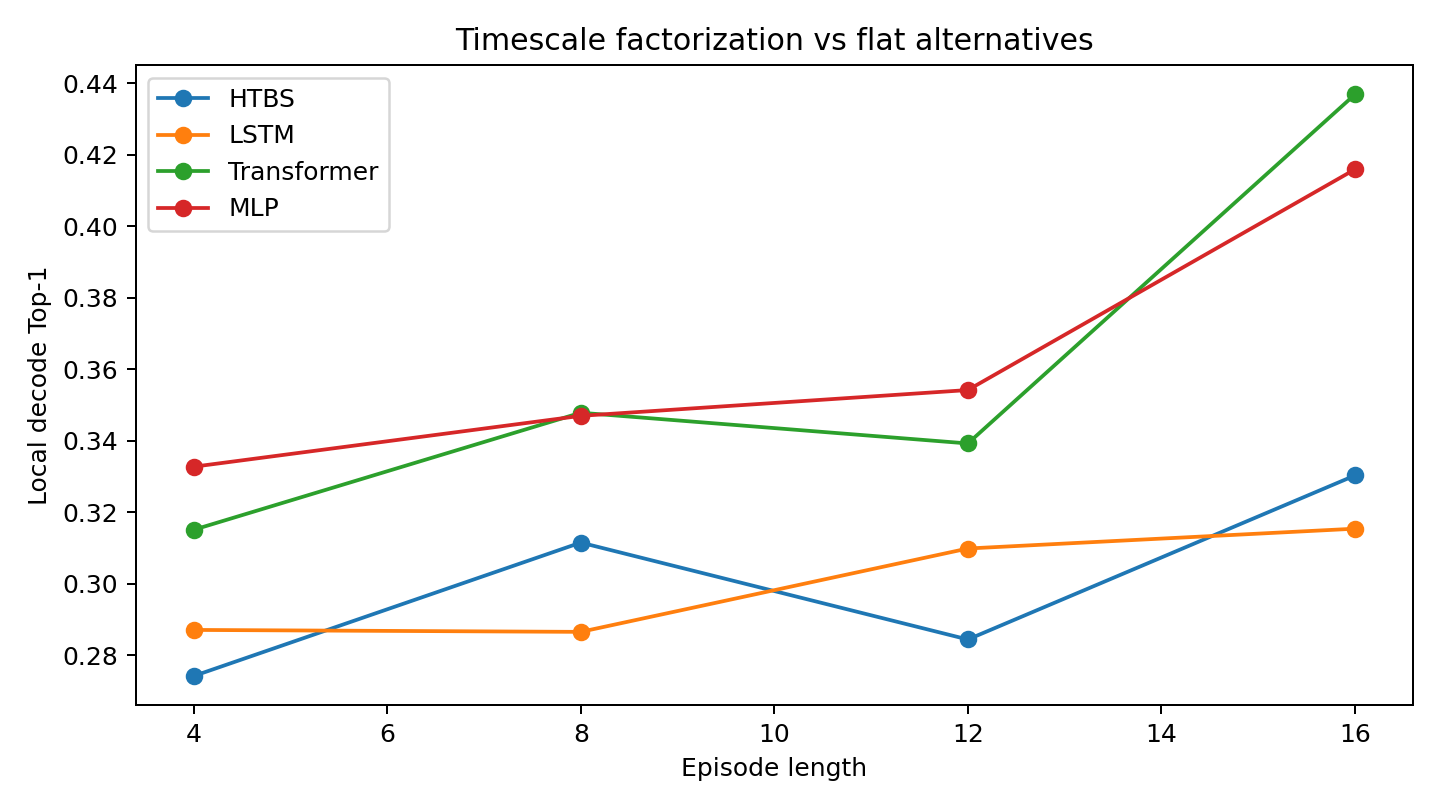
\includegraphics[width=0.82\linewidth]{../results/figures/exp4_timescale.png}
\caption{Local Top-1 accuracy across sequence lengths. HTBS is competitive at longer horizons but does not dominate.}
\label{fig:timescale}
\end{figure}

This is the most sobering result in the paper. HTBS never clearly wins the experiment. At length 16 it reaches Top-1 0.3303, but the transformer still does better at 0.4369. Even the per-step MLP is hard to beat at shorter horizons. The right conclusion is not that multiscale compression is useless; it is that the present HTBS design does not yet earn a superiority claim.

\subsection{Sparse commitment}
\begin{table}[H]
\centering
\caption{Dense versus sparse predictive commitment.}
\begin{tabular}{lccc}
\toprule
Model / subset & Cosine & Local Top-1 & Local Top-5 \\
\midrule
Dense predictor & 0.5443 & 0.3353 & 0.5728 \\
Sparse blended output & 0.6145 & 0.3533 & 0.7253 \\
Sparse committed subset & 0.6272 & 0.5931 & 0.9411 \\
\bottomrule
\end{tabular}
\label{tab:sparse}
\end{table}

\begin{table}[H]
\centering
\caption{Gate behavior at a 30\% target commitment rate.}
\begin{tabular}{lc}
\toprule
Statistic & Value \\
\midrule
Mean gate probability & 0.2916 \\
Actual commitment rate & 0.3000 \\
High-change commitment rate & 0.3599 \\
Low-change commitment rate & 0.2622 \\
Committed Top-1 minus dense Top-1 & 0.2567 \\
\bottomrule
\end{tabular}
\label{tab:sparse-gate}
\end{table}

\begin{figure}[H]
\centering
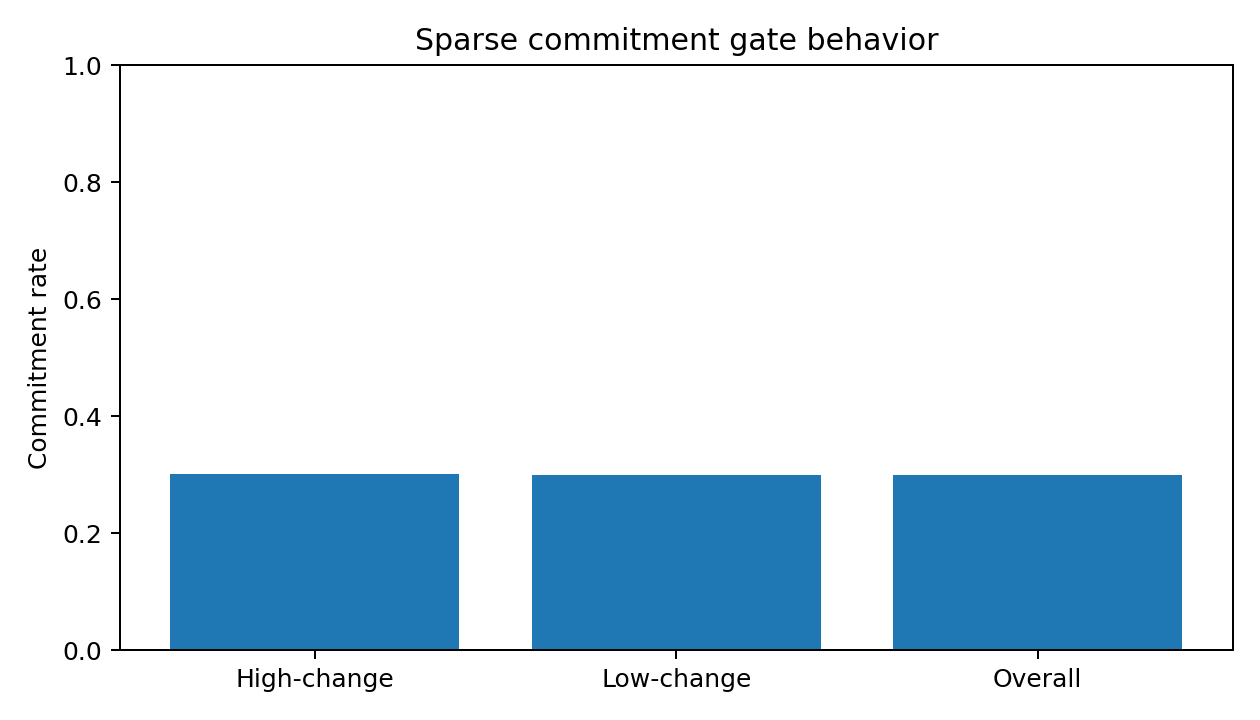
\includegraphics[width=0.72\linewidth]{../results/figures/exp5_sparse.png}
\caption{Commitment rates for the sparse gate.}
\label{fig:sparse}
\end{figure}

SPCG reaches the target average budget almost exactly, and the committed subset attains Top-1 0.5931 versus 0.3353 for the dense baseline, a gain of 0.2567. That is the good news. The bad news is that the gate still does not cleanly separate event boundaries from routine transitions: the high-minus-low commitment-rate gap is 9.77\%. So the compute-allocation story looks real, but the stronger event-boundary interpretation remains limited.

\subsection{Focused TICP follow-up}
\begin{table}[H]
\centering
\caption{Twin-stream follow-up across three held-out action splits. Numbers report gains of twin-stream over single-stream on held-out actions.}
\begin{tabular}{lcc}
\toprule
Held-out split & Cosine gain & Top-1 gain \\
\midrule
pickup+toggle & 0.0178 & 0.0268 \\
turning & 0.0131 & 0.0076 \\
forward+drop & 0.0211 & 0.0245 \\
\bottomrule
\end{tabular}
\label{tab:ticp-followup}
\end{table}

\begin{figure}[H]
\centering
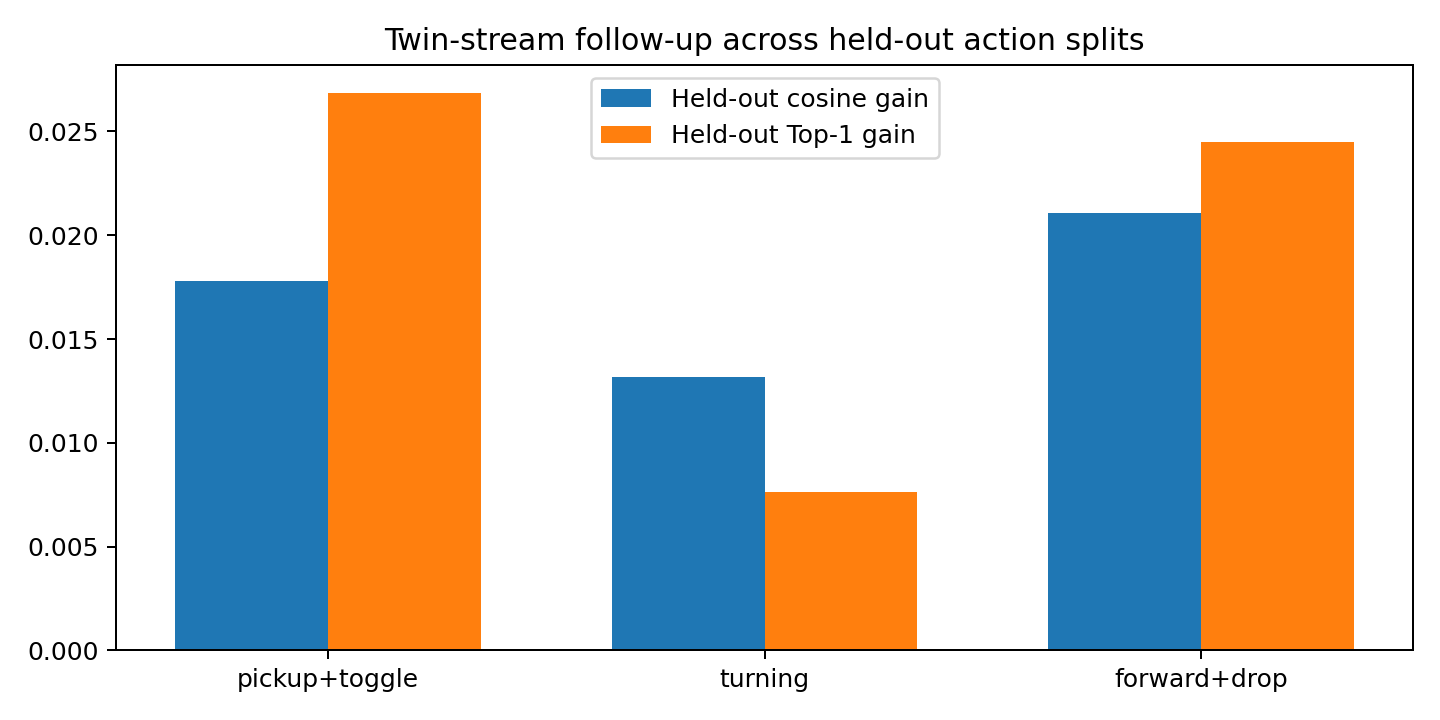
\includegraphics[width=0.82\linewidth]{../results/figures/exp6_ticp_followup.png}
\caption{Twin-stream follow-up across three held-out action splits. The improvement is modest but consistently positive.}
\label{fig:ticp-followup}
\end{figure}

The follow-up experiment is important because it checks whether the main TICP result was a lucky split. It was not. Across all three held-out partitions, the twin-stream model improves held-out cosine and held-out Top-1 over the single-stream baseline. The gains are not dramatic, but they are consistent: +0.0178/+0.0268 for pickup+toggle, +0.0131/+0.0076 for turning, and +0.0211/+0.0245 for forward+drop. That consistency strengthens the paper's strongest claim more than any further rhetorical polishing could.

\section{Discussion}
The experiments support three different conclusions of three different strengths.

First, bounded external state is a clear win. The retrieval and workspace experiments both reinforce the original systems argument that long-horizon agents should not rely on transcript growth alone. The retrieval result is especially instructive because it is slightly inconvenient: lexical matching remains the strongest shallow retriever on LoCoMo. That makes the paper more credible, not less.

Second, explicit action/world decomposition helps. The held-out-action BabyAI experiment is not a giant effect, but it is the most coherent positive finding in the repo. More importantly, the follow-up across three alternate held-out action splits keeps the sign of the result positive every time. That does not prove causal reasoning in the full Pearlian sense, but it does justify taking TICP seriously as the core novel component.

Third, the other two CWE components need more work. HTBS is plausible and sometimes competitive, but the baselines do not collapse as sequence length increases. SPCG can budget computation and isolate a high-accuracy committed subset, yet it does not cleanly learn prediction-error boundaries. In other words, there is a paper here, but not the triumphant version.

\section{Limitations}
This project has several obvious limitations.
\begin{itemize}
    \item The intervention results come from small offline BabyAI trajectories, not from a large embodied agent stack.
    \item The action generalization setup relies on text embeddings of action names. That is a reasonable semantic prior, but it is still a design choice rather than a law of nature.
    \item HTBS was tested only in one concrete implementation with GRU cells and mean pooling. A stronger multiscale design might perform differently.
    \item The sparse gate was evaluated with a threshold chosen to match the target commitment rate; this makes budget control explicit, but it also means the evaluation is not a pure emergent-boundary story.
    \item The paper does not claim a full causal model in Pearl's formal sense. CWE is better described as an intervention-aware predictive architecture.
\end{itemize}

\section{Conclusion}
CWE is not a wholesale replacement for transformers, and this paper does not pretend otherwise. The honest result is narrower: action-effect factorization is useful, bounded state reconstruction is useful, and the specific multiscale and sparse-gating mechanisms tested here are promising but not yet decisive. That is still enough for a solid systems paper, because it turns a vague architectural intuition into a reproducible set of wins, failures, and next steps.

\bibliographystyle{plainnat}
\bibliography{references}

\end{document}
